% XeLaTeX can use any Mac OS X font. See the setromanfont command below.
% Input to XeLaTeX is full Unicode, so Unicode characters can be typed directly into the source.

% The next lines tell TeXShop to typeset with xelatex, and to open and save the source with Unicode encoding.

%!TEX TS-program = xelatex
%!TEX encoding = UTF-8 Unicode

\documentclass[12pt]{article}
\newcommand\tab[1][1cm]{\hspace*{#1}}
\usepackage{geometry}                % See geometry.pdf to learn the layout options. There are lots.
\geometry{letterpaper}                   % ... or a4paper or a5paper or ... 
%\geometry{landscape}                % Activate for for rotated page geometry
%\usepackage[parfill]{parskip}    % Activate to begin paragraphs with an empty line rather than an indent
\usepackage{graphicx}
\usepackage{amssymb}
\usepackage{amsmath}
\usepackage{mathtools}
\usepackage{float}
\usepackage{graphicx}




\usepackage{fontspec,xltxtra,xunicode}
\defaultfontfeatures{Mapping=tex-text}
\setromanfont[Mapping=tex-text]{Hoefler Text}
\setsansfont[Scale=MatchLowercase,Mapping=tex-text]{Gill Sans}
\setmonofont[Scale=MatchLowercase]{Andale Mono}

\title{CS 375 HW1}
\author{Baptiste Saliba}

\begin{document}
\large
\maketitle

“I have done this assignment completely on my own. I have not copied it, nor have I given my solution to anyone else. I understand that if I am involved in plagiarism or cheating I will have to sign an official form that I have cheated and that this form will be stored in my official university record. I also understand that I will receive a grade of 0 for the involved assignment for my first offense and that I will receive a grade of “F” for the course for any additional offense.”\\

\pagebreak
Question 1:
Set: $[3,4,5,8] $ find subsets that sum to 13\\
\begin{figure}[ht]
  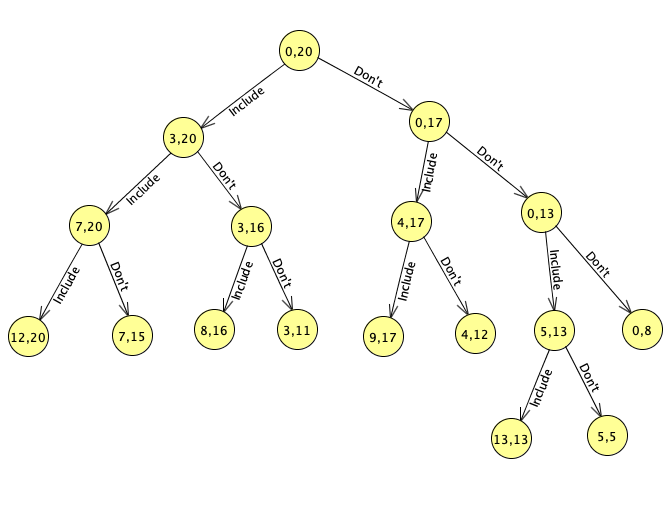
\includegraphics[width=\linewidth]{Q1.png}
\end{figure}\\
Optimal: \{5, 8\} or Item 3 and 4\\ 

\pagebreak

Question 2: 
\begin{figure}[ht]
  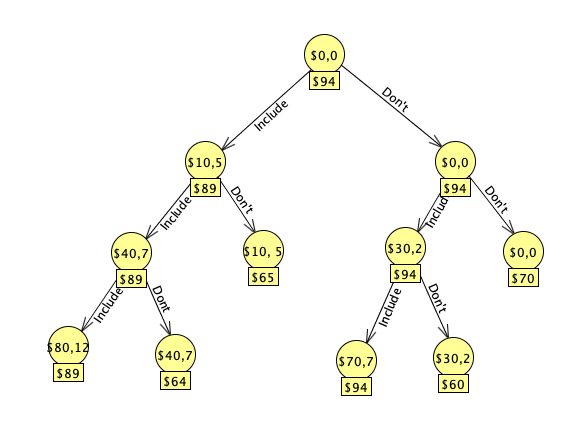
\includegraphics[width=\linewidth]{Q2.png}
\end{figure}

\pagebreak
Question 3:\\
\tab Sorted:\\
\tab Item 1: \$30, 2lb, \$15/lb\\
\tab Item 2: \$40, 5lb, \$8/lb\\
\tab Item 3: \$30, 10lb, \$3/lb\\
\tab Item 4: \$10, 5lb, \$2/lb
\begin{figure}[ht]
  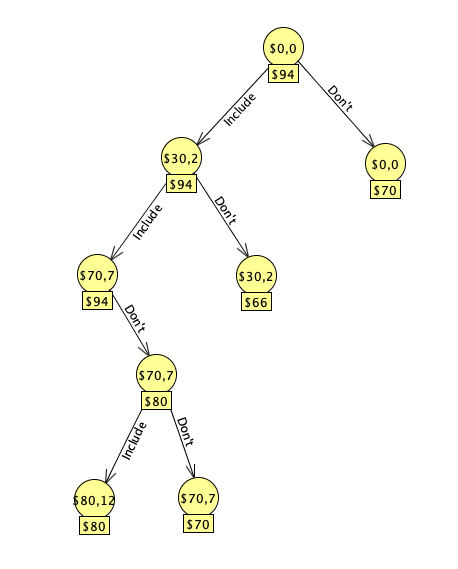
\includegraphics[width=11.7cm]{Q3.png}
\end{figure}\\

\pagebreak
Question 4:
\begin{center}
\begin{tabular}{|c|c|c|c|c|}
\hline
$Node Added$ & $D(a) nearest$ & $D(b) nearest$ &$D(c) nearest$ & $D(d) nearest$ \\
\hline
$\{\}$ & $\infty /NILL$ & $\infty /NILL$ & $\infty /NILL$ & $\infty /NILL$ \\
\hline
$\{a\}$ &  & $8/a$ & $1/a$ & $\infty /NILL$ \\
\hline
$\{a,c\}$ &  & $3/c$ &  & $5/c$ \\
\hline
$\{a,c,b\}$ &  &  &  & $2/b$ \\
\hline
\end{tabular}\\
\end{center}

Question 5:\\
\tab Note: formatted as "x(y)" where x is the weight and y is the order picked
\begin{figure}[ht]
  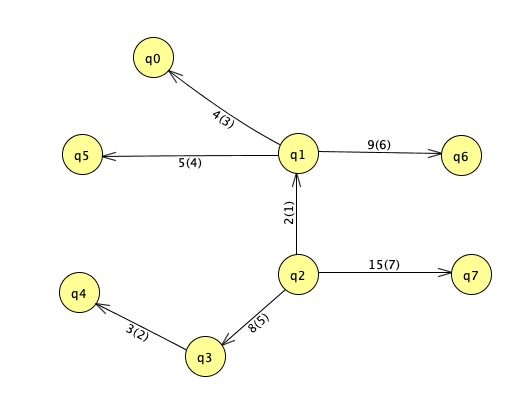
\includegraphics[width=\linewidth]{Q4.png}
\end{figure}\\
Total Weight = 2+3+4+5+8+9+15 = 46\\

Question 6:\\\\\\
$D(0) = $
\begin{tabular}{|cccc|}
\hline
$0$ & $8$ & $?$ & $1$\\
$?$ & $0$ & $1$ & $?$\\
$4$ & $?$ & $0$ & $?$\\
$?$ & $2$ & $9$ & $0$\\
\hline
\end{tabular}\\\\\\
$D(1) = $
\begin{tabular}{|cccc|}
\hline
$0$ & $8$ & $?$ & $1$\\
$?$ & $0$ & $1$ & $?$\\
$4$ & $12$ & $0$ & $5$\\
$?$ & $2$ & $9$ & $0$\\
\hline
\end{tabular}\\\\\\
$D(2) = $
\begin{tabular}{|cccc|}
\hline
$0$ & $8$ & $9$ & $1$\\
$?$ & $0$ & $1$ & $?$\\
$4$ & $12$ & $0$ & $5$\\
$?$ & $2$ & $3$ & $0$\\
\hline
\end{tabular}\\\\\\
$D(3) = $
\begin{tabular}{|cccc|}
\hline
$0$ & $8$ & $9$ & $1$\\
$5$ & $0$ & $1$ & $6$\\
$4$ & $12$ & $0$ & $5$\\
$7$ & $2$ & $3$ & $0$\\
\hline
\end{tabular}\\\\\\
$D(4) = $
\begin{tabular}{|cccc|}
\hline
$0$ & $3$ & $4$ & $1$\\
$5$ & $0$ & $1$ & $6$\\
$4$ & $7$ & $0$ & $5$\\
$7$ & $2$ & $3$ & $0$\\
\hline
\end{tabular}\\\\\\
\end{document}  